\documentclass{IEEEtran}

\usepackage{cite}
\usepackage{amsmath}
\usepackage{amssymb}
\usepackage{url}
\usepackage{graphicx}
\usepackage{booktabs}
\usepackage{microtype}
\usepackage[table]{xcolor}
\usepackage{tikz}
\usetikzlibrary{positioning,arrows.meta,fit,backgrounds}
\usepackage[hidelinks]{hyperref}

\definecolor{PhaseGreen}{RGB}{45,176,150}
\definecolor{PhaseBlue}{RGB}{52,190,255}
\definecolor{PhasePurple}{RGB}{126,87,194}
\definecolor{PhaseOrange}{RGB}{245,166,35}
\definecolor{SoftGray}{RGB}{86,100,126}
\definecolor{SoftInk}{RGB}{33,42,62}
\definecolor{DeepNavy}{RGB}{11,26,51}
\definecolor{PaleGray}{RGB}{244,248,252}

\title{A Fairness-Aware Sequential Routing Framework for Clinical Diagnostic Workflows and Quantum Routing\\[0.3em]
{\large\textit{Comparing Multi-Armed, Contextual, and Informative Bandit Methods}}}

\author{%
\begin{minipage}{0.48\textwidth}
\begin{center}
{\bf Piter Z. Garcia}\\
\begin{small}
MS Data Science / Decision-Making \& Algorithmic Fairness\\
Rochester Institute of Technology (RIT)\\
{\it pizg8794@g.rit.edu}
\end{small}
\end{center}
\end{minipage}
\hfill
\begin{minipage}{0.48\textwidth}
\begin{center}
{\bf Dr. Daniel Krutz, Travis Desell}\\
\begin{small}
Department of Software Engineering, Data Science\\
RIT Research Advisors\\
{\it dxkvse@g.rit.edu, tjdvse@g.rit.edu}
\end{small}
\end{center}
\end{minipage}%
}

\begin{document}
\maketitle
\vspace{-0.7em}

\section{Approach Overview}
This work proposes a shared fairness-aware sequential routing framework for two domain-distinct settings: clinical diagnostic workflows and quantum-network routing. The common ground is routing under scarcity. In the clinical setting, the policy routes patients, tests, and escalation effort through a diagnostic pathway; in the quantum setting, the policy routes entanglement and limited network resources through candidate paths. In both cases, unfair routing is not only an equity failure but also a performance failure. When one subgroup is systematically routed through weaker tests, slower escalation paths, or less reliable network allocations, the result is directly measurable degradation in outcomes such as false negatives, delayed intervention, delivery success, and latency.

A concrete clinical workflow illustrates the point. A patient may first receive a low-cost screen, then a confirmatory test, and finally an escalation decision when the evidence remains uncertain. If some populations enter that sequence with missing history, noisier biomarkers, or delayed follow-up information, then the routing policy may repeatedly choose weaker next steps for those patients even when average system utility appears acceptable. In that setting, fairness must be defined through sequential outcome gaps, such as false-negative disparities or delayed-escalation disparities, because the harm appears through the path a patient is routed through rather than through a single isolated prediction.

A parallel quantum workflow makes the same logic visible in a second technical setting. A controller must repeatedly choose paths and allocate scarce entanglement or qubit resources under probabilistic link success, congestion, and changing network state. If some flow groups are repeatedly routed through lower-quality links or are consistently deprioritized when resources are scarce, unfairness appears as service inequity in success probability, waiting time, or latency. This is why the project treats quantum fairness as an allocation consequence rather than as a loose analogy to clinical fairness: in both settings, unfair routing determines who receives reliable service and who repeatedly absorbs system failure.

The method family is therefore organized as a deliberate comparison spectrum rather than as a single preferred algorithm. Multi-armed bandits provide a low-information routing baseline, contextual bandits test whether observed side information improves routing quality, and informative-context methods test whether richer but still imperfect information reduces disparity or merely relocates it. The research target is not simply average reward maximization. It is fairness under uneven context quality, partial feedback, and shift, measured during learning over time. Pairing the two domains under one routing framework is valuable because it allows the same fairness-aware decision logic to be tested in a socially critical diagnostic setting and in an emerging high-impact networking setting that is already pushing toward breakthrough infrastructure.

\section{Domain Model and Interaction Logic}
Figure~\ref{fig:domain_model} presents the shared domain model as four color-coded phases. \textbf{Phase 1} defines the routing setting through either a clinical workflow or a quantum network. \textbf{Phase 2} forms the routing context and makes visible the fairness driver of degraded or uneven information. \textbf{Phase 3} applies the policy family to choose a routing action, such as test escalation or path allocation. \textbf{Phase 4} records partial feedback, utility, and fairness, then feeds those results into mitigation and comparison. The phased presentation matters because the assignment requires the diagram to explain both the major stages and the interaction among their components, not merely to decorate the page.

\begin{figure*}[!t]
\centering
\resizebox{0.98\textwidth}{!}{%
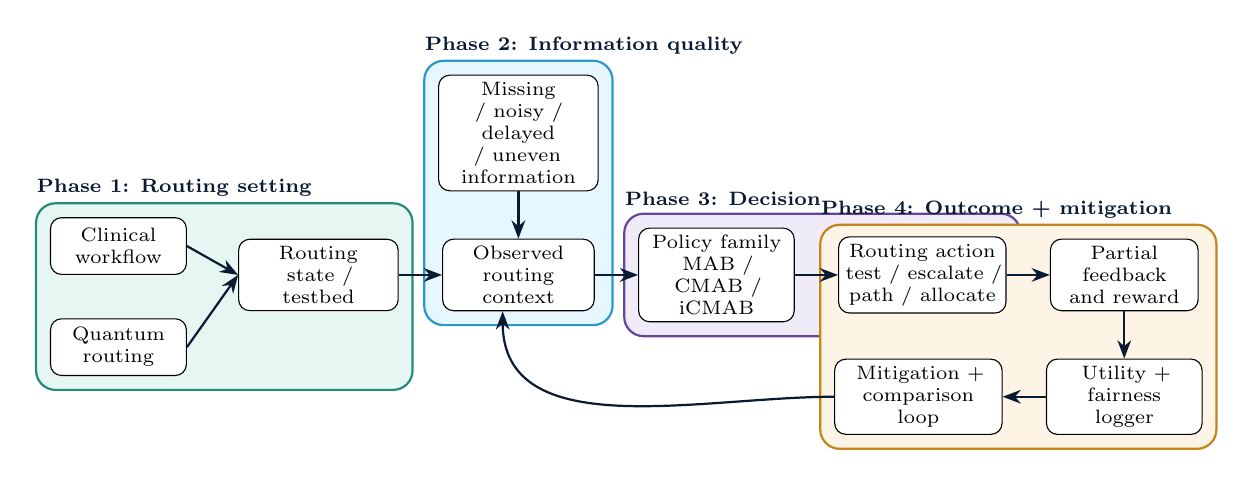
\begin{tikzpicture}[
font=\scriptsize,
box/.style={draw, rounded corners=4pt, align=center, text width=1.55cm, minimum height=0.72cm, inner sep=2.5pt, fill=white},
arr/.style={-Stealth, thick, draw=DeepNavy},
phase/.style={draw, rounded corners=7pt, inner sep=5pt, thick},
phaselabel/.style={font=\scriptsize\bfseries, text=DeepNavy, anchor=west}
]
\node[box] (clin) {Clinical\\workflow};
\node[box, below=0.55cm of clin] (quant) {Quantum\\routing};
\node[box, right=0.65cm of clin.south east, anchor=west, text width=1.85cm] (env) {Routing\\state /\\testbed};
\node[box, right=0.55cm of env, text width=1.75cm] (ctx) {Observed routing\\context};
\node[box, above=0.60cm of ctx, text width=1.85cm] (deg) {Missing / noisy /\\delayed / uneven\\information};
\node[box, right=0.55cm of ctx, text width=1.80cm] (pol) {Policy family\\MAB / CMAB / iCMAB};
\node[box, right=0.55cm of pol, text width=1.95cm] (act) {Routing action\\test / escalate /\\path / allocate};
\node[box, right=0.55cm of act, text width=1.70cm] (fb) {Partial feedback\\and reward};
\node[box, below=0.60cm of fb, text width=1.80cm] (log) {Utility + fairness\\logger};
\node[box, left=0.55cm of log, text width=1.95cm] (mit) {Mitigation +\\comparison loop};

\begin{scope}[on background layer]
\node[phase, fill=PhaseGreen!12, draw=PhaseGreen!80!black, fit=(clin)(quant)(env)] (p1) {};
\node[phase, fill=PhaseBlue!12, draw=PhaseBlue!80!black, fit=(ctx)(deg)] (p2) {};
\node[phase, fill=PhasePurple!12, draw=PhasePurple!80!black, fit=(pol)(act)] (p3) {};
\node[phase, fill=PhaseOrange!12, draw=PhaseOrange!80!black, fit=(fb)(log)(mit)] (p4) {};
\end{scope}

\node[phaselabel] at ([xshift=-0.10cm,yshift=0.18cm]p1.north west) {Phase 1: Routing setting};
\node[phaselabel] at ([xshift=-0.10cm,yshift=0.18cm]p2.north west) {Phase 2: Information quality};
\node[phaselabel] at ([xshift=-0.10cm,yshift=0.18cm]p3.north west) {Phase 3: Decision};
\node[phaselabel] at ([xshift=-0.10cm,yshift=0.18cm]p4.north west) {Phase 4: Outcome + mitigation};

\draw[arr] (clin.east) -- (env.west);
\draw[arr] (quant.east) -- (env.west);
\draw[arr] (env) -- (ctx);
\draw[arr] (deg) -- (ctx);
\draw[arr] (ctx) -- (pol);
\draw[arr] (pol) -- (act);
\draw[arr] (act) -- (fb);
\draw[arr] (fb) -- (log);
\draw[arr] (log) -- (mit);
\draw[arr] (mit.west) to[out=180,in=270] ([xshift=-0.20cm]ctx.south);
\end{tikzpicture}%
}
\caption{Color-coded shared domain model. The same four phases support both settings while preserving domain-specific meanings for routing state, action, reward, and fairness metrics.}
\label{fig:domain_model}
\end{figure*}

The interaction logic follows the figure from left to right. In Phase 1, the environment or testbed creates the decision state: either a clinical case moving through a diagnostic pathway or a quantum network state containing candidate paths and resource constraints. In Phase 2, the system observes only the information available at decision time. That is why the degraded-context mechanism is separated as its own stage in the diagram. It represents missing, noisy, delayed, or uneven information quality, which is the main fairness driver studied by the project. In the clinical branch, this may correspond to incomplete patient history, delayed tests, or subgroup-dependent measurement quality. In the quantum branch, it may correspond to stale link estimates, partial congestion information, or uncertainty about available resources.

In Phase 3, the policy family converts imperfect information into a routing action. This is where the method spectrum matters. The non-contextual baseline shows what happens when routing decisions rely mostly on empirical action values, the contextual baseline shows what changes when side information is incorporated directly, and the informative-context extension tests whether better information access changes both utility and fairness behavior. In Phase 4, the environment reveals only partial feedback for the chosen action, after which the logger records reward, utility, and group disparity over time. The mitigation and comparison loop then asks the exact question at the center of the project: whether richer context, fairness-aware policy updates, or both are needed to improve the routing process.

These decisions relate directly to the domain model. The domains are not collapsed into one application because their actions, operational constraints, and fairness metrics remain different. Clinical routing evaluates outcomes such as false-negative gaps, intervention delay, and resource cost, whereas quantum routing evaluates service-equity gaps such as differential success and latency across flow groups. However, they still belong in one framework because the same interaction logic links routing state, imperfect context, action choice, partial feedback, and fairness logging in both settings. That is the reason the implementation plan can follow from one diagram while still preserving distinct testbed semantics.

\section{Why This Design}
This design is stronger than simpler alternatives for four reasons. First, the clinical branch is simulation-first by design, not by limitation. That choice allows controlled experiments with missingness, delay, noise, subgroup-specific context degradation, and intervention costs without depending on sensitive patient records or on a dataset that already fixes the decision path in advance. Second, the quantum branch builds on an existing routing and resource-allocation foundation rather than inventing a toy second problem. That gives the second testbed technical credibility and keeps the work aligned with real constraints that matter in emerging network systems.

Third, the method spectrum is necessary because the project is studying how fairness changes as routing decisions gain access to more information. A contextual-only study would make it impossible to tell whether context actually improves fairness relative to a simpler low-information baseline. A single best-model study would reduce the work to algorithm selection rather than analysis of fairness formation. A post-hoc fairness audit would also be insufficient, because the central claim is that disparity can appear during exploration, adaptation, and repeated routing under partial feedback. For that reason, fairness must be measured during learning and mitigation must be tested inside the same sequential loop rather than after the decisions have already been made.

Fourth, the shared cross-domain design is better than two isolated projects. A single clinical study could motivate social importance but would say less about whether the framework captures a broader class of routing problems. A single quantum study could motivate technical novelty but would risk looking detached from direct human impact. Bringing the domains together creates a stronger research argument: unfair routing harms both people and systems, and a framework that can expose those harms across two very different settings is more defensible than a narrow one-domain claim. The project therefore gains two forms of value at once. It can identify performance failures that are directly tied to fairness, and it can position those findings as guidance for both current systems and future fairness-aware routing technologies.

This also addresses why the work should be done this way instead of following what is already common in the literature around each separate domain. The existing landscape is strong in pieces but fragmented in structure: clinical fairness work often emphasizes offline prediction or pipeline-specific auditing, while routing work often emphasizes throughput, robustness, or threat response before fairness. The present design deliberately connects these strands through one online comparison framework. That integrated framing is one of its main advantages because it turns fairness from a downstream reporting metric into a first-class property of routing quality, implementation design, and system evaluation.

\section{Implementation Plan}
The implementation plan follows directly from the phased domain model rather than from a disconnected checklist. The clinical branch will build a simulation environment for sequential diagnostic routing, including screening, confirmatory testing, retesting, and escalation under subgroup-sensitive differences in observed context. The quantum branch will integrate a routing and resource-allocation environment for repeated path selection and entanglement or qubit assignment under probabilistic links, congestion, and changing network conditions. Both testbeds will be exposed through a shared policy interface so that the same method spectrum can be evaluated in comparable experimental rounds.

Reward and metric design will be domain-specific but structurally aligned. On the utility side, the framework will track measures such as diagnostic accuracy, intervention cost, routing success, and latency. On the fairness side, it will track disparities that reflect how routing quality differs across groups, including false-negative or delayed-escalation gaps in the clinical setting and success-rate or latency disparities across flow groups in the quantum setting. These metrics will be logged per step and summarized over time so that the project can distinguish transient unfairness during learning from persistent unfairness after longer runs.

The implementation decisions also support reproducibility, which is part of the credibility of the approach. The project will use fixed random seeds, explicit configuration files, modular experiment runs, and small sanity-check settings that make it possible to validate the framework without a long execution barrier. The software package will also expose the common policy interface, metric logger, and testbed stepping logic in a way that supports unit or integration testing before large comparisons are run. At least one fairness-aware mitigation mechanism will then be evaluated within the same framework so that the final analysis can compare baseline unfairness, mitigation effects, and utility-fairness tradeoffs under both routing settings. In that sense, the implementation plan is the operational consequence of Figure~\ref{fig:domain_model}: each build step corresponds to one stage of the shared routing architecture.

\begin{thebibliography}{9}\setlength{\itemsep}{0em}
\bibitem{garcia2025equitable_bioinformatics}
Garcia, P. Z. Equitable Bioinformatics: Enhancing Diagnostic Decision-Making through {RNA}
and Biomarker Data. Course paper (ISTE 780 Phase 4), Rochester Institute of Technology,
2025.
\bibitem{garcia2026threat_aware_quantum_routing}
Garcia, P. Z. Threat-Aware Evaluation of Quantum Entanglement Routing and Qubit Allocation
via Hybrid Contextual Bandits. Unpublished manuscript (GA-Work internal draft), Rochester
Institute of Technology, 2026.
\end{thebibliography}

\end{document}
